\section{Limitation of Past Surveys}\label{sec:past_detection_context}
   
   What is apparent from the plethora of debris disk studies over the last three decades is the differences in the reported incidence rate of excesses. Though there is a consensus in terms of typical rates for a given spectral type at various stellar ages, the differences, even within these different bins, require further consideration.
   
   There are a few reasons why these differences exist. The first is instrument sensitivity. Different instruments aboard these satellites are sensitive to a certain degree. A good review can be found in \citet{Wyatt2008}, where Dr. Wyatt describes the limiting fractional excess $R_{\lambda,\rm{lim}}$ above which a disk is detectable, typically calculated based on the limits of the faintest disk detected in the survey. Thus, equation 11 in \citet{Wyatt2008} defines the lowest fractional luminosity above which a disk is detectable
   
   \begin{equation}\label{eq:detection_limits}
   f_{\rm{det}} = 6\times10^9 X_\lambda \frac{R_{\lambda,{\rm lim}}L_\star}{r^2 T_\star^4} \frac{B_\lambda(T_\star)}{B_\lambda(T_d)}. 
   \end{equation}
   
    %===================================================================
    %  DISK DETECTION
    %===================================================================
    \begin{figure}
    \centering
    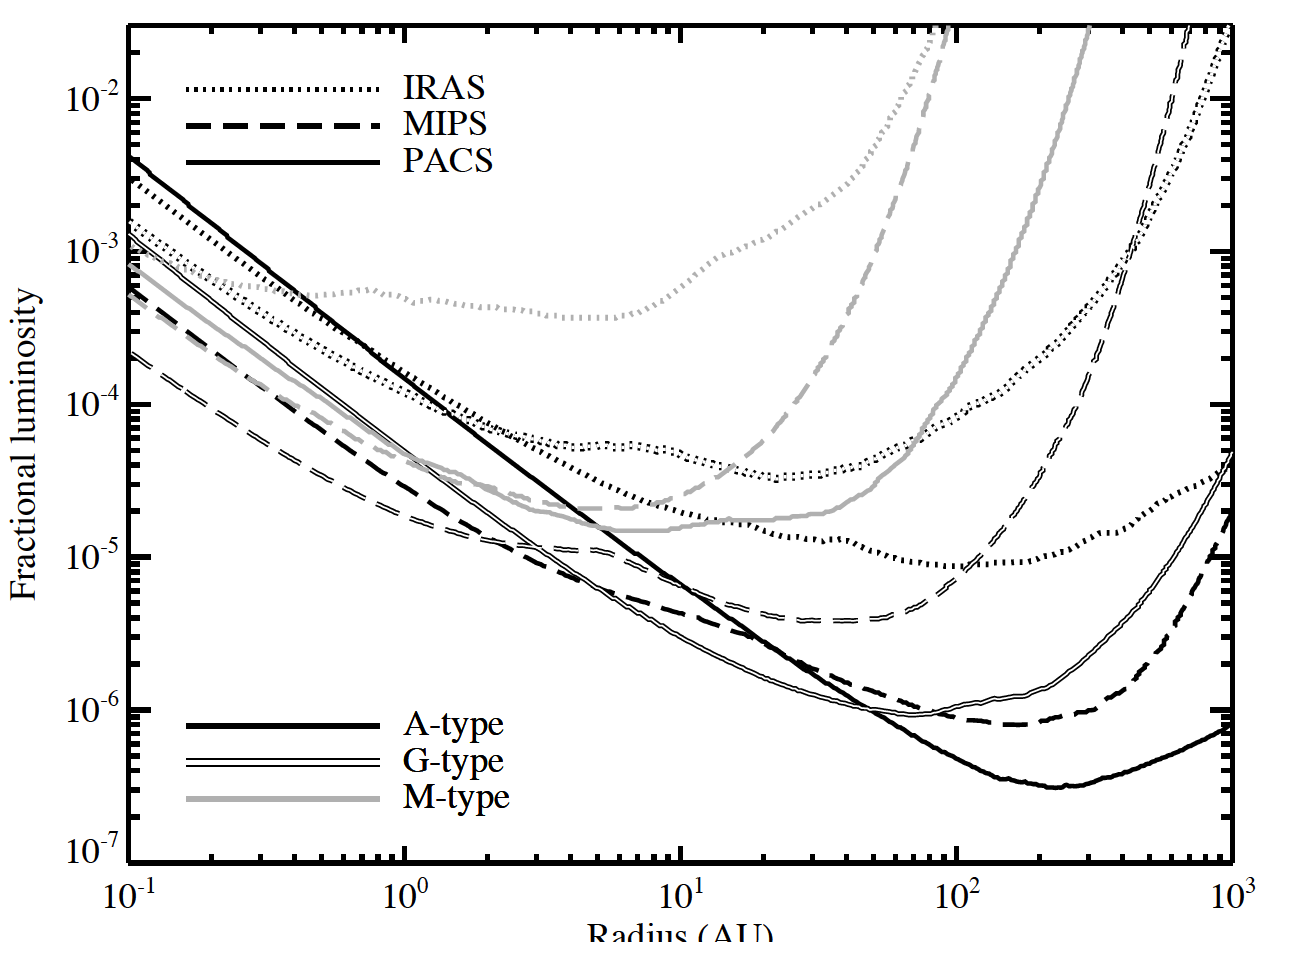
\includegraphics[scale=0.2]{Ch2/Detection_limits_Kennedy}
    \caption[Sensitivity Limits of Cold Disk Surveys]{This plot shows the limiting fractional luminosity as a function of distance from the star based on data from the DEBRIS survey. Above these lines, 25\% of the stars in DEBRIS were detected by surveys conducted by \iras\, Spitzer/MIPS (24 and 70\micron) and Herschel/PACS (100 and 160\micron) \citep[Image credit: Grant Kennedy in][]{Matthews2014}}
    \label{fig:detection_limits}
    \end{figure}
    %===================================================================
    
   
   Figure~\ref{fig:detection_limits} shows the limiting fractional luminosity from a few different surveys as a function of radius from the star. From \iras\ to Herschel, improvements in both detector technology and an increase in mirror size have allowed for the detection of fainter and fainter dust populations. Hence, the increase of incidence rates from \iras\ to Spitzer does not come as much of a surprise given that Spitzer is sensitive to fainter dust (cold or warm). Differences in incidence rates can also arise due to the threshold of an excess some studies may adopt compared to others. 
   
   As explained in \S~\ref{sec:excess_resolvedimaging}, the excess flux is determined from the measured IR flux subtracted from the photospheric flux in the IR, which is extrapolated from model fits to optical and near-IR flux measurements. Studies may determine the significance of an excess detection from this subtraction on a case by case basis, or from the statistical significance based on the distribution of a large survey. The former method can under or overestimate the excess if significant flux variations occur between the epoch of observations between the optical data and the IR data, while the latter technique may introduce large false-discovery rates \textbf{check this} as well as reduce the sensitivity of fainter disks for small samples in a survey. 
   
   Studies that used some of the more notable space based observatories like Herschel or Spitzer were limited to sample sizes of $\sim$500 stars, due to the pointed nature of the satellite. And although \iras\ was an all-sky mission, it also produced a couple hundred excess sources. The study by \citet{Rhee2007} searched for excesses around tens of thousands of Hipparcos main-sequence stars, and produced roughly 50 new excesses, the majority of which were still cold disk detections. We have seen that cold dust is easier to detect due to the large contrast with the photosphere in the far-IR. Low contrast becomes an issue in the mid-IR, where there are a relatively small number of warm dust detections.
   
   The small number of warm dust detections is due to the small coverage of very sensitive pointed satellites like Spitzer and Herschel, and the relatively low resolution and sensitivity of the last all-sky mission, \iras, where the resolution of the \iras\ beam was 30'' at 12\micron. Thus, to address these limitations, I now shift focus of this thesis to finding warm dust with the latest all-sky infrared mission: the Wide-Field Infrared Survey Explorer Spacecraft.
   
   
\section{The Wide-Field Infrared Survey Explorer\\ Mission}\label{sec:wise_intro}

    The success of the \iras\ mission was one of the motivations for launching another new and improved infrared all-sky mission. The goals of the Wide-Field Infrared Survey Explorer mission \citep[WISE;][]{Wright2010} were to observe the entire sky at two near-IR and two mid-IR wavelengths, thus improving and complementing the achievements of \iras\. In this section, I discuss the details of the WISE mission. Analysis of data from the \WS\ survey constitutes the bulk of my thesis. In the following section, I will summarize the \WS\ mission, explain its purpose and technical specifications, and discuss how data from the mission can be used to identify circumstellar dust. 
   

    \subsection{Mission Overview}\label{sec:wise_overview}


    \WS\ is an Earth orbiting observatory, 525~km above the Earth's surface. \WS\ is funded by NASA/JPL and launched on December 14th, 2009. It is a medium-class explorer mission weighing 750~kg. The satellite consists of a 40~cm diameter telescope and four imaging CCDs which are cooled by solid hydrogen cryostats. Two of the CCDs are designed to image the sky in the near-infrared wavelengths (3.5\micron\ and 4.6\micron) and two in the mid-infrared (12\micron\ and 22\micron). Figure~\ref{fig:WISE_Satellite} shows an illustration of the physical satellite. 
  
    
    %===================================================================
    %  WISE SATELLITE
    %===================================================================
    \begin{figure}
    \centering
    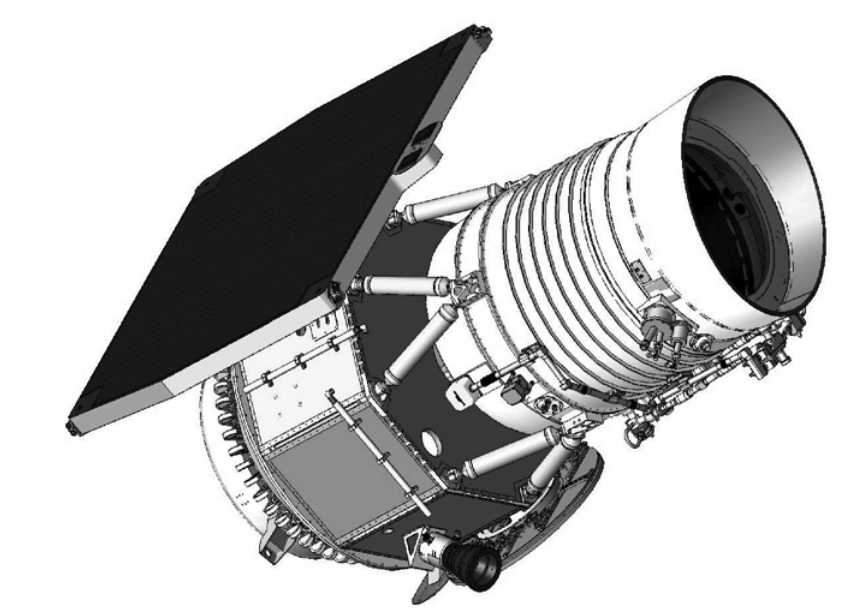
\includegraphics[width=\textwidth]{Ch2/wise_satellite}
    \caption[\WS\ Satellite]{Illustration of the \WS\ satellite.}
    \label{fig:WISE_Satellite}
    \end{figure}
    %===================================================================
    
 
    The mission was successful in scanning 99.99\% of the entire sky in the aforementioned IR bands. WISE's detector field-of-view is 47' on a side. During its continual orbit around the Earth, overlapping observation frames 11 second cadences were taken (8.8~s of integration). The overlap of frames, over multiple orbits, ensures greater depth of coverage. In one day, the satellite performs 15 orbits. Figure~\ref{fig:wise_scan_plan} shows the overlapping frames as the satellite orbits the Earth. Further details of the entire mission can be found online\footnote{\url{http://wise2.ipac.caltech.edu/docs/release/allsky/expsup/}} or in \citet{Wright2010}. 

    %===================================================================
    %  WISE SCAN PLAN
    %===================================================================
    \begin{figure}
    \centering
    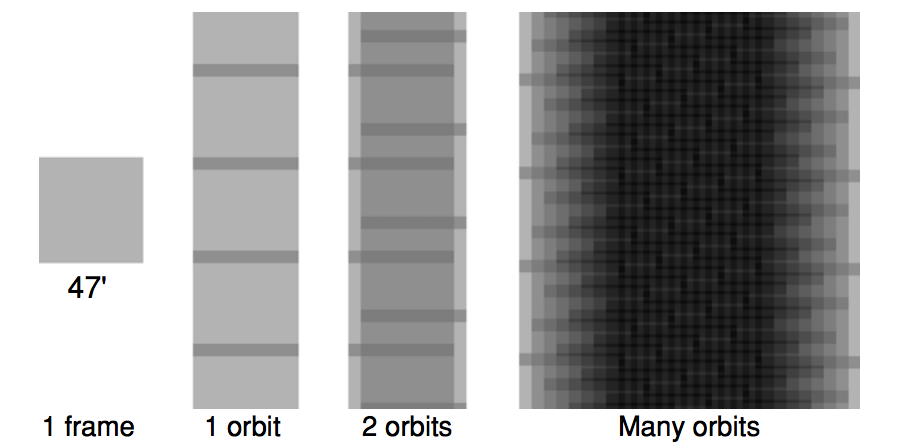
\includegraphics[width=\textwidth]{Ch2/wise_scan_plan}
    \caption[\WS\ Sky Coverage]{\WS\ coverage evolution over many orbits of the satellite around Earth. Each frame is a cadence of 11~s, and subsequent observations provide overlapping regions between frames. Lighter to darker shades of gray indicate increasing depth of coverage. Image taken from \citet{Wright2010}.}
    \label{fig:wise_scan_plan}
    \end{figure}
    %===================================================================
    
    
   
   
    \subsection{WISE Bands}\label{sec:wise_bands}

    %===================================================================
    %  WISE BANDS
    %===================================================================
    \begin{figure}
    \centering
    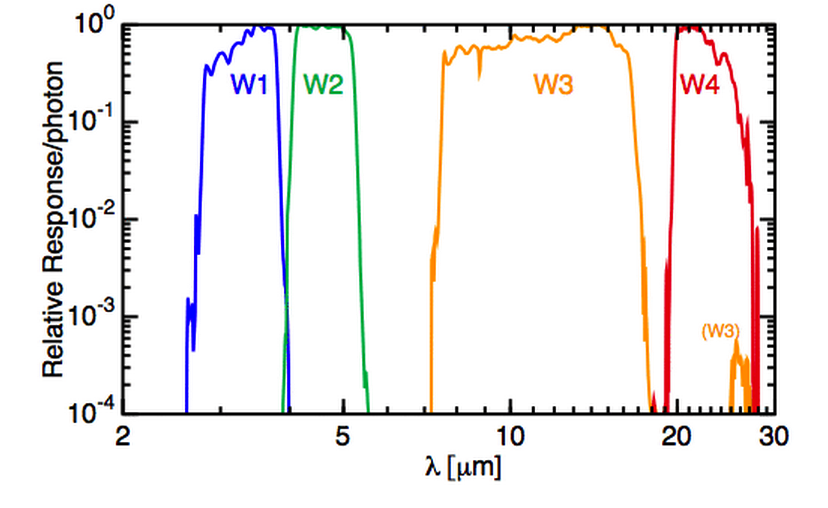
\includegraphics[scale=0.5]{Ch2/wise_response}
    \caption[\WS\ Bands]{Relative spectral response curves for all four \WS\ bands. Plot was taken from the WISE Explanatory Supplement.}
    \label{fig:wise_bands}
    \end{figure}
    %===================================================================
   
   
   The two near-IR channels image the sky at band centered wavelengths of 3.4\micron\ and 4.6\micron\ using HgCdTe arrays, each with 18\micron\ 1024 $\times$ 1024 pixels. Both of these detectors are cooled to 32~K. The mid-IR channel detectors image the sky at band centered wavelengths of 12\micron\ and 22\micron\ and are made from Si:As BIB arrays of the same structure as the near-IR channels. These arrays are cooled to a temperature of 8.2~K. For the remainder of this thesis, I will refer to each of these bands as $W1$ (3.4\micron), $W2$ (4.6\micron), $W3$ (12\micron) and $W4$ (22\micron). Figure~\ref{fig:wise_bands} shows the relative spectral response of each of the detectors. 
   
    
    
   
    \subsection{\WS\ Data Releases}

    The WISE mission has produced a number of different data releases. The first release, called the \textit{WISE Preliminary Release} was made public on April 14, 2011\footnote{\url{http://wise2.ipac.caltech.edu/docs/release/prelim/preview.html}} and contained data that covered only 57\% of the sky. The next public release of WISE data was made on March 14, 2012. This data set was called the \textit{All-Sky Data Release}\footnote{\url{http://wise2.ipac.caltech.edu/docs/release/allsky/}} and covered the entire sky in all four bands. After the cryostats were depleted, WISE began its ``warm'' mission, and only collected data in the two near-IR $W1$ and $W2$ bands. This commenced the Near-Earth Object WISE (NEOWISE) mission. A subsequent all-sky data release by WISE came on November 13, 2013 called the \textit{All-WISE Data Release}\footnote{\url{http://wise2.ipac.caltech.edu/docs/release/allwise/}}. For the work I present in the rest of this dissertation, I only use measurements from the \textit{All-Sky Data Release}, except in comparison with other release. 
    
    Since the WISE data is in the public domain, it can easily be accessed online. The online databases consists of measurements for over half a billion objects in all four bands. These measurements consist of photometric data for each band, as well as meta-data pertaining to the quality of the data product. The database also consists of Atlas images of the processed data and can be viewed at \url{http://irsa.ipac.caltech.edu/applications/wise/}. 
    
    \subsection{Cautionary Tales of WISE Data}\label{sec:bad_wise}
    
    Before simply using the \WS\ data products, it is important to understand all the nuances and aspects of what one might encounter in this data. For instance, the \WS\ team implemented profile-fitting algorithms to extract the standard reported measurements and uncertainties. The \WS\ data also provides several meta-data tags for each source to characterize the quality of the measurement. Here I will summarize some of the more important meta-data tags found in the \WS\ database. All of these pertain to identifying sources whose photometry have a high probability of contamination from artificial and astrophysical sources, and hence are likely to bias the presence of an IR excess (i.e., debris disk).
    
        \subsubsection{Extended Source Contamination}
    
    The Two Micron All-Sky Survey \citep[\mass\ ;][]{Skrutskie2006} is a ground based all-sky survey that has mapped out the entire sky in three near-IR bands: $J$ (1.25\micron), $H$ (1.6\micron), and $K_s$ (2.17\micron). As a result, the location of known extragalatic extended sources is well known in the near-IR. Stars whose photometry might be contaminated by the flux from a nearby \mass\ extended source are flagged in \WS\ using \verb|ext_flg| meta-data tag. Figure~\ref{fig:extflg_contamination} shows clearly that the photometry of the star, HIP~3293, is contaminated from the isophotal footprint of a nearby \mass\ galaxy. 
            
        %===================================================================
        %  2MASS CONTAMINATION
        %===================================================================
        \begin{figure}[!h]
        \centering
        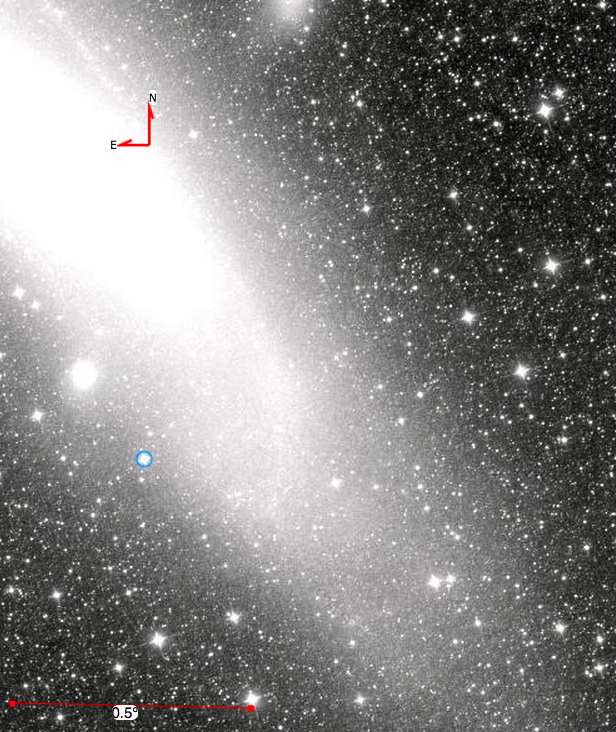
\includegraphics[width=0.4\textwidth]{Ch2/extflg_2_HIP3293}
        \caption[Contamination From \mass\ Extended Source.]{An example of a star contaminated due to a \mass\ extended source object. This $W4$ band image shows the star, HIP~3293, indicated by the blue circle, within the vicinity of a background extragalactic source. The photometry of this star is flagged with \textit{extflg}=2, indicating that it is within the isophotal footprint of this galaxy, and is likely to be contaminated.}
        \label{fig:extflg_contamination}
        \end{figure}
        %===================================================================
        
    
        
    
        \subsubsection{Artificial Instrument Contamination}
    Source photometry is also likely to be contaminated by artificial optical artifacts.  Diffraction spikes from nearby bright sources, scattered light halo's from the edge of a bright source's PSF, optical ghosts caused by internal reflections of the telescope optics, and latent images can all contaminate a real source or give rise to an spurious object. The level of contamination for a source in each of the four \WS\ bands is given  the confusion flag \verb|cc_flg| --- a four character string. For instance, the star HIP~32362's \verb|cc_flg=hhdd|, implying that the $W1$ and $W2$ bands are predominantly contaminated by halo artifcats from a nearby bright star, while the $W3$ and $W4$ bands are contaminated by diffraction spikes from a nearby bright source. Figure~\ref{fig:ccflag_contamination} shows HIP~32362, with markers for the location of the different artifacts. A full description of these artifacts can be found in Section IV.4.g of the \WS\ Explanatory Supplement\footnote{\url{http://wise2.ipac.caltech.edu/docs/release/allsky/expsup/sec4_4g.html}}. 
        
        
        %===================================================================
        %  CONFUSION FLAG CONTAMINATION
        %===================================================================
        \begin{figure}[!h]
        \centering
        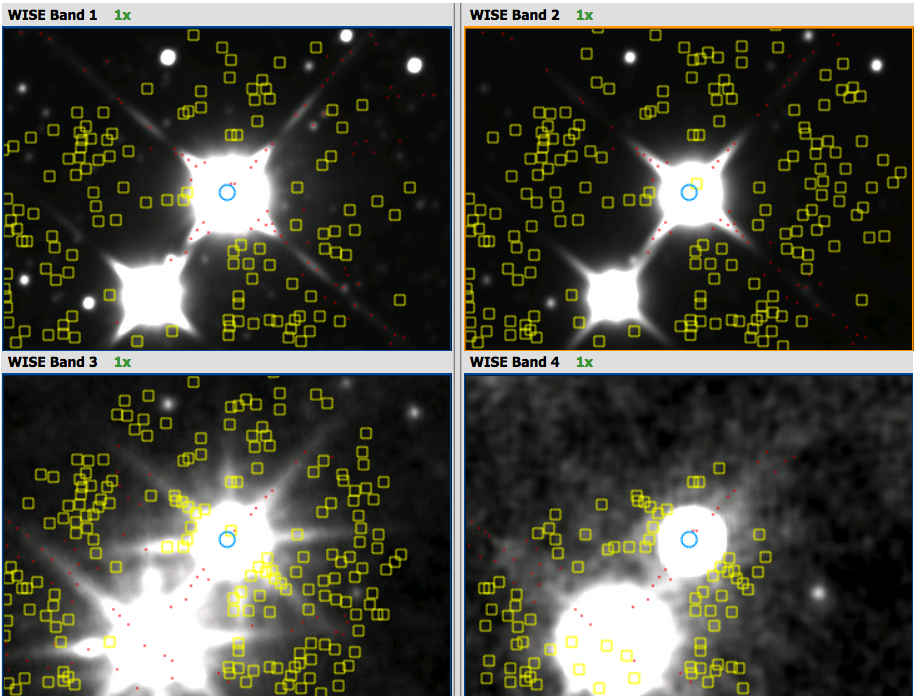
\includegraphics[width=\textwidth]{Ch2/ccflag_hhdd_HIP32362}
        \caption[Contamination From Optical Articats]{\WS\ four band image centered on HIP~32362. The confusion flag for this star is \textit{ccflg=hhdd}. These flags, one character per band indicate that the source is real but is most likely contaminated by mostly halo (h) or from diffraction spikes (d) from a nearby bright star. Diffraction spikes and halo artifacts are marked by red circles and yellow squares, respectively.}
        \label{fig:ccflag_contamination}
        \end{figure}
        %===================================================================
        
    
        \subsubsection{Moon Contamination}
        
        \WS's earth orbit unfortunately meant it had to contend with scattered light from the Moon. \WS's observing pattern was such that it attempted to avoid this scattered light. However, complete avoidance was impossible, and the scattered light from the Moon heavily affected frames in $W3$ and $W4$ relative to the near-IR bands. Figure~\ref{fig:moonflag_contamination} shows the structure of this effect in the $W3$ and $W4$ band images, with the star HIP~114340 marked for reference. The level of the contamination is given by the \verb|moon_flg| and provides the percentage of single frames that are contaminated by the moon for each band. Additional information on Moon contamination in \WS\ can be found at \url{http://wise2.ipac.caltech.edu/docs/release/allsky/expsup/sec6_2.html}.
        
        %===================================================================
        %  MOON FLAG CONTAMINATION
        %===================================================================
        \begin{figure}[!h]
        %\centering
        \begin{tabular}{cc}
        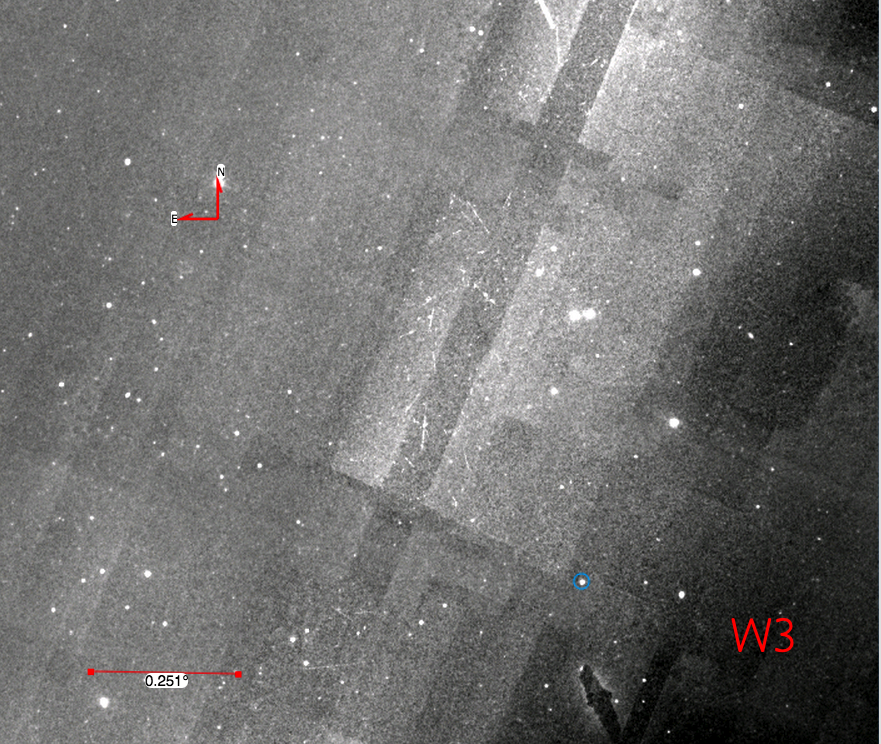
\includegraphics[width=0.6\textwidth]{Ch2/moonflg_HIP114340_W3_88}&
        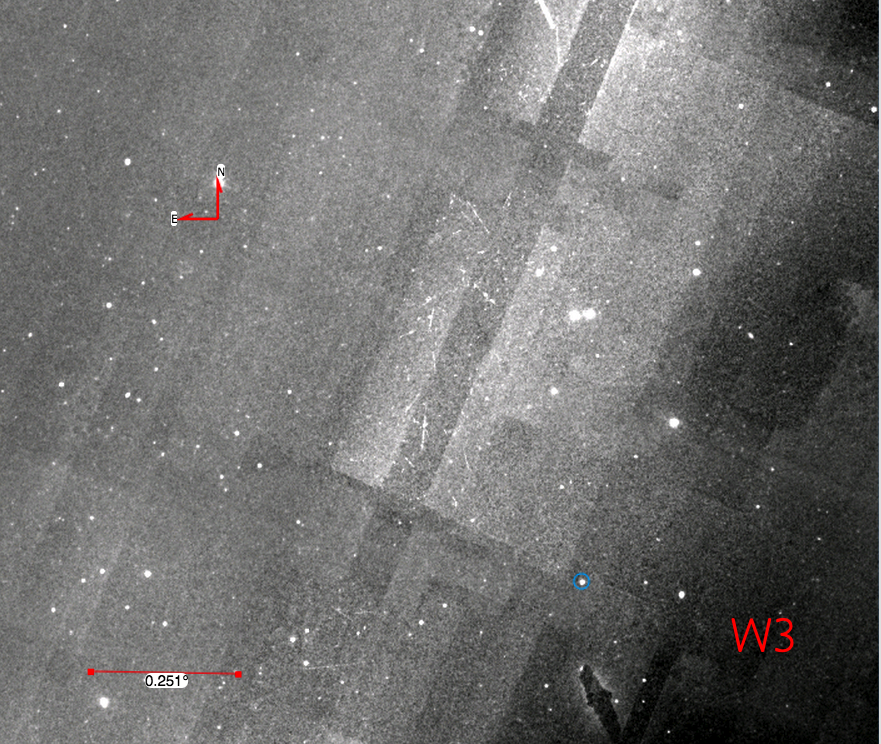
\includegraphics[width=0.6\textwidth]{Ch2/moonflg_HIP114340_W3_88}
        \end{tabular}
        \caption[]{}
        \label{fig:moonflag_contamination}
        \end{figure}
        %===================================================================
    
    
        \subsubsection{Saturated WISE Photometry}
    The detectors CCDs aboard the \WS\ spacecraft saturate for relatively bright sources: 8.1~mag, 6.7~mag, 3.8~mag, and -0.4~mag in $W1$, $W2$, $W3$, and $W4$, respectively. It is important to keep these limits in mind, as the photometry for sources brighter than these saturation limits are unreliable. Additional information on the saturation of \WS\ sources can be found in Section VI.3.d of the \WS\ Explanatory Supplement\footnote{\url{http://wise2.ipac.caltech.edu/docs/release/allsky/expsup/sec6_3d.html}}. 
    
    However, the profile-fitting algorithm attempts to obtain measurements of saturated sources by using non-saturated pixels in the wings of the source's PSF. As a result, a systematic trend arises as a function of the source brightness. Figure 17 in Section IV.4.a.vi.1 illustrates this trend of source brightness as a function of \mass\ $K_s-WISE$ color. This trend is stronger in $W1$ and $W2$, which are the limiting bands in searching for excesses. As I will show in Chapter 3, these trends can be corrected, and thus allow for brighter stars to be used in a large survey. 
    
    
        \subsubsection{Internally Inconsistent Variability}
    
    The variability flag in the \WS\ database \verb|var_flg| indicates the probability that the photometry in a particular band is variable. The variability may be due to intrinsic astrophysical processes, although this is typically reserved for non-main sequence objects. The variability may also be due to a number of different factors pertaining to instrumental artifacts between subsequent single frame observations by \WS. Additional information for the variability flag can be found at \url{http://wise2.ipac.caltech.edu/docs/release/allsky/expsup/sec4_4ciii6.html}
    
        \subsubsection{Internally Inconsistent Photometry}
    
    During the course of this project, we found a peculiar behavior in the \WS\ data. In some very rare cases, the final reported flux measurement in the All-Sky database --- after all relevant single frames for that particular star were coadded by the \WS\ internal algorithms --- significantly differed from the averaged single-frame measured fluxes for the same star. In other words, there seemed to be internal \WS\ inconsistencies in the measurements of a small percentage of stars. Since we are looking for peculiar (i.e., excesses), we are sensitive to finding these stars. This behavior will also bias the level of the measured flux. Although there is no reported reason for this phenomenon, we have found a way to deal with this inconsistency and detail it in \S~2.3 of Chapter 3. 
    

    \subsection{Advantages Over Previous Debris Disk Surveys}

    As outlined in \S~\ref{sec:excess_resolvedimaging}, detection of an IR excess from a debris disk requires precise and accurate measurement of the photospheric flux. In other words, this boils down to a survey which is sensitive to low levels of dust emission. This is especially important when searching for warm dust as the contrast between the thermal dust and stellar photospheric emission is lowest. One also has to be able to discern whether the IR excess is associated with the star system. This in turn requires high resolution to remove sources of astrophysical confusion. In addition, the incidence rate of excesses established by the last few decades of debris disk studies have shown that unless the star is young, there is a low probability of detecting an excess. The number of young associations in the nearby Solar neighborhood is relatively low (reference and maybe a number). Hence surveying field stars for excesses requires a large sample size to detect a greater number of sources. 
    %===================================================================
    %  Mission Sensitivities
    %===================================================================
    \begin{figure}
    \centering
    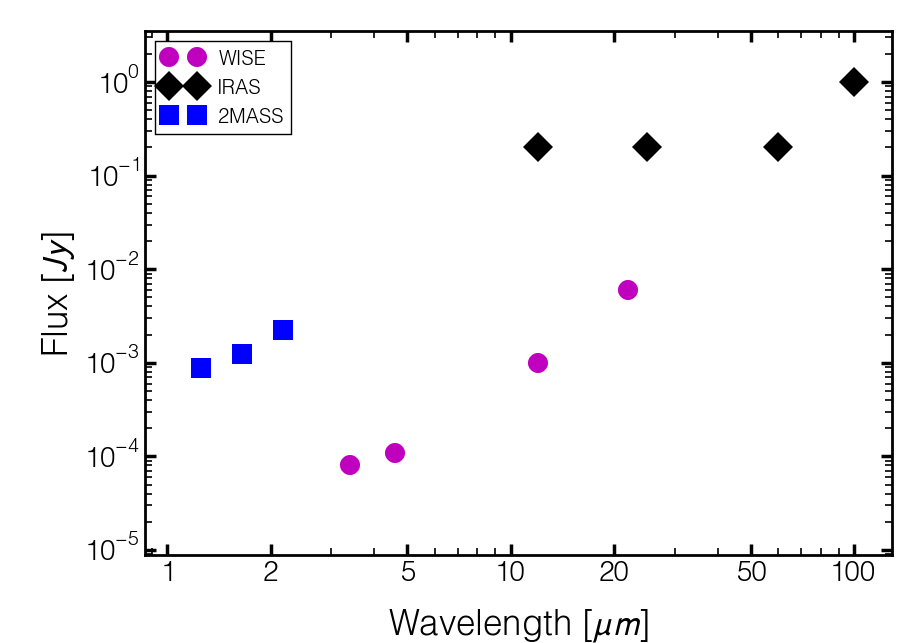
\includegraphics[scale=0.5]{Ch2/flux_density_comparison}
    \caption[]{}
    \label{fig:flux_comparison}
    \end{figure}
    %===================================================================
    

    
    \iras' all-sky design made it ideal to to search for excesses around a large number of stars. And though it found a few hundred excesses, its successor --- WISE --- is capable of advancing this search. This is due to two reasons. The first is that WISE is a more sensitive survey compared to \iras. \iras\ was sensitive down to $\sim$0.2~Jy in its 12 and 25\micron\ bands. In comparison, WISE is 160--200$\times$ more sensitive in its $W3$ and $W4$ bands. Figure~\ref{fig:flux_comparison} shows the absolute sensitivity of both \iras\ and WISE for each of their IR detectors. The second reason why WISE has the ability to outperform \iras\ in the mid-IR is due to WISE's relatively high resolution compared to \iras. WISE's angular resolution for $W1$--$W4$ is 6.1'', 6.4'', 6.5'', and 12'', respectively, with an astrometric accuracy of 0.2''. In comparison, the angular resolution of the 12\micron\ detector is 30'' but has a positional accuracy of 20''. Figure~\ref{fig:region_compare} shows the same patch of sky in \textbf{region in milky way} seen by \iras\ and WISE at 12\micron. The comparison images clearly show that with the superior angular resolution, WISE has the ability to identify a plethora of unconfused debris disks from their IR excesses. This is also reflected in the sheer number of point sources catalogued in the WISE All-Sky Database ($\sim$600,000,000), compared to those in the \iras\ database ($\sim$270,000). 
    
    %===================================================================
    %  \iras\ VS. WISE Images
    %===================================================================
    %\begin{figure}
    %\centering
    %\includegraphics[scale=0.5]{Ch2/region_compare}
    %\caption[]{}
    %\label{fig:region_compare}
    %\end{figure}
    %===================================================================
    
    
    
    
    %===================================================================
    %  \iras\ VS. WISE VS SPITZER MIPS24 SENSITIVITY
    %===================================================================
    \begin{figure}
    \centering
    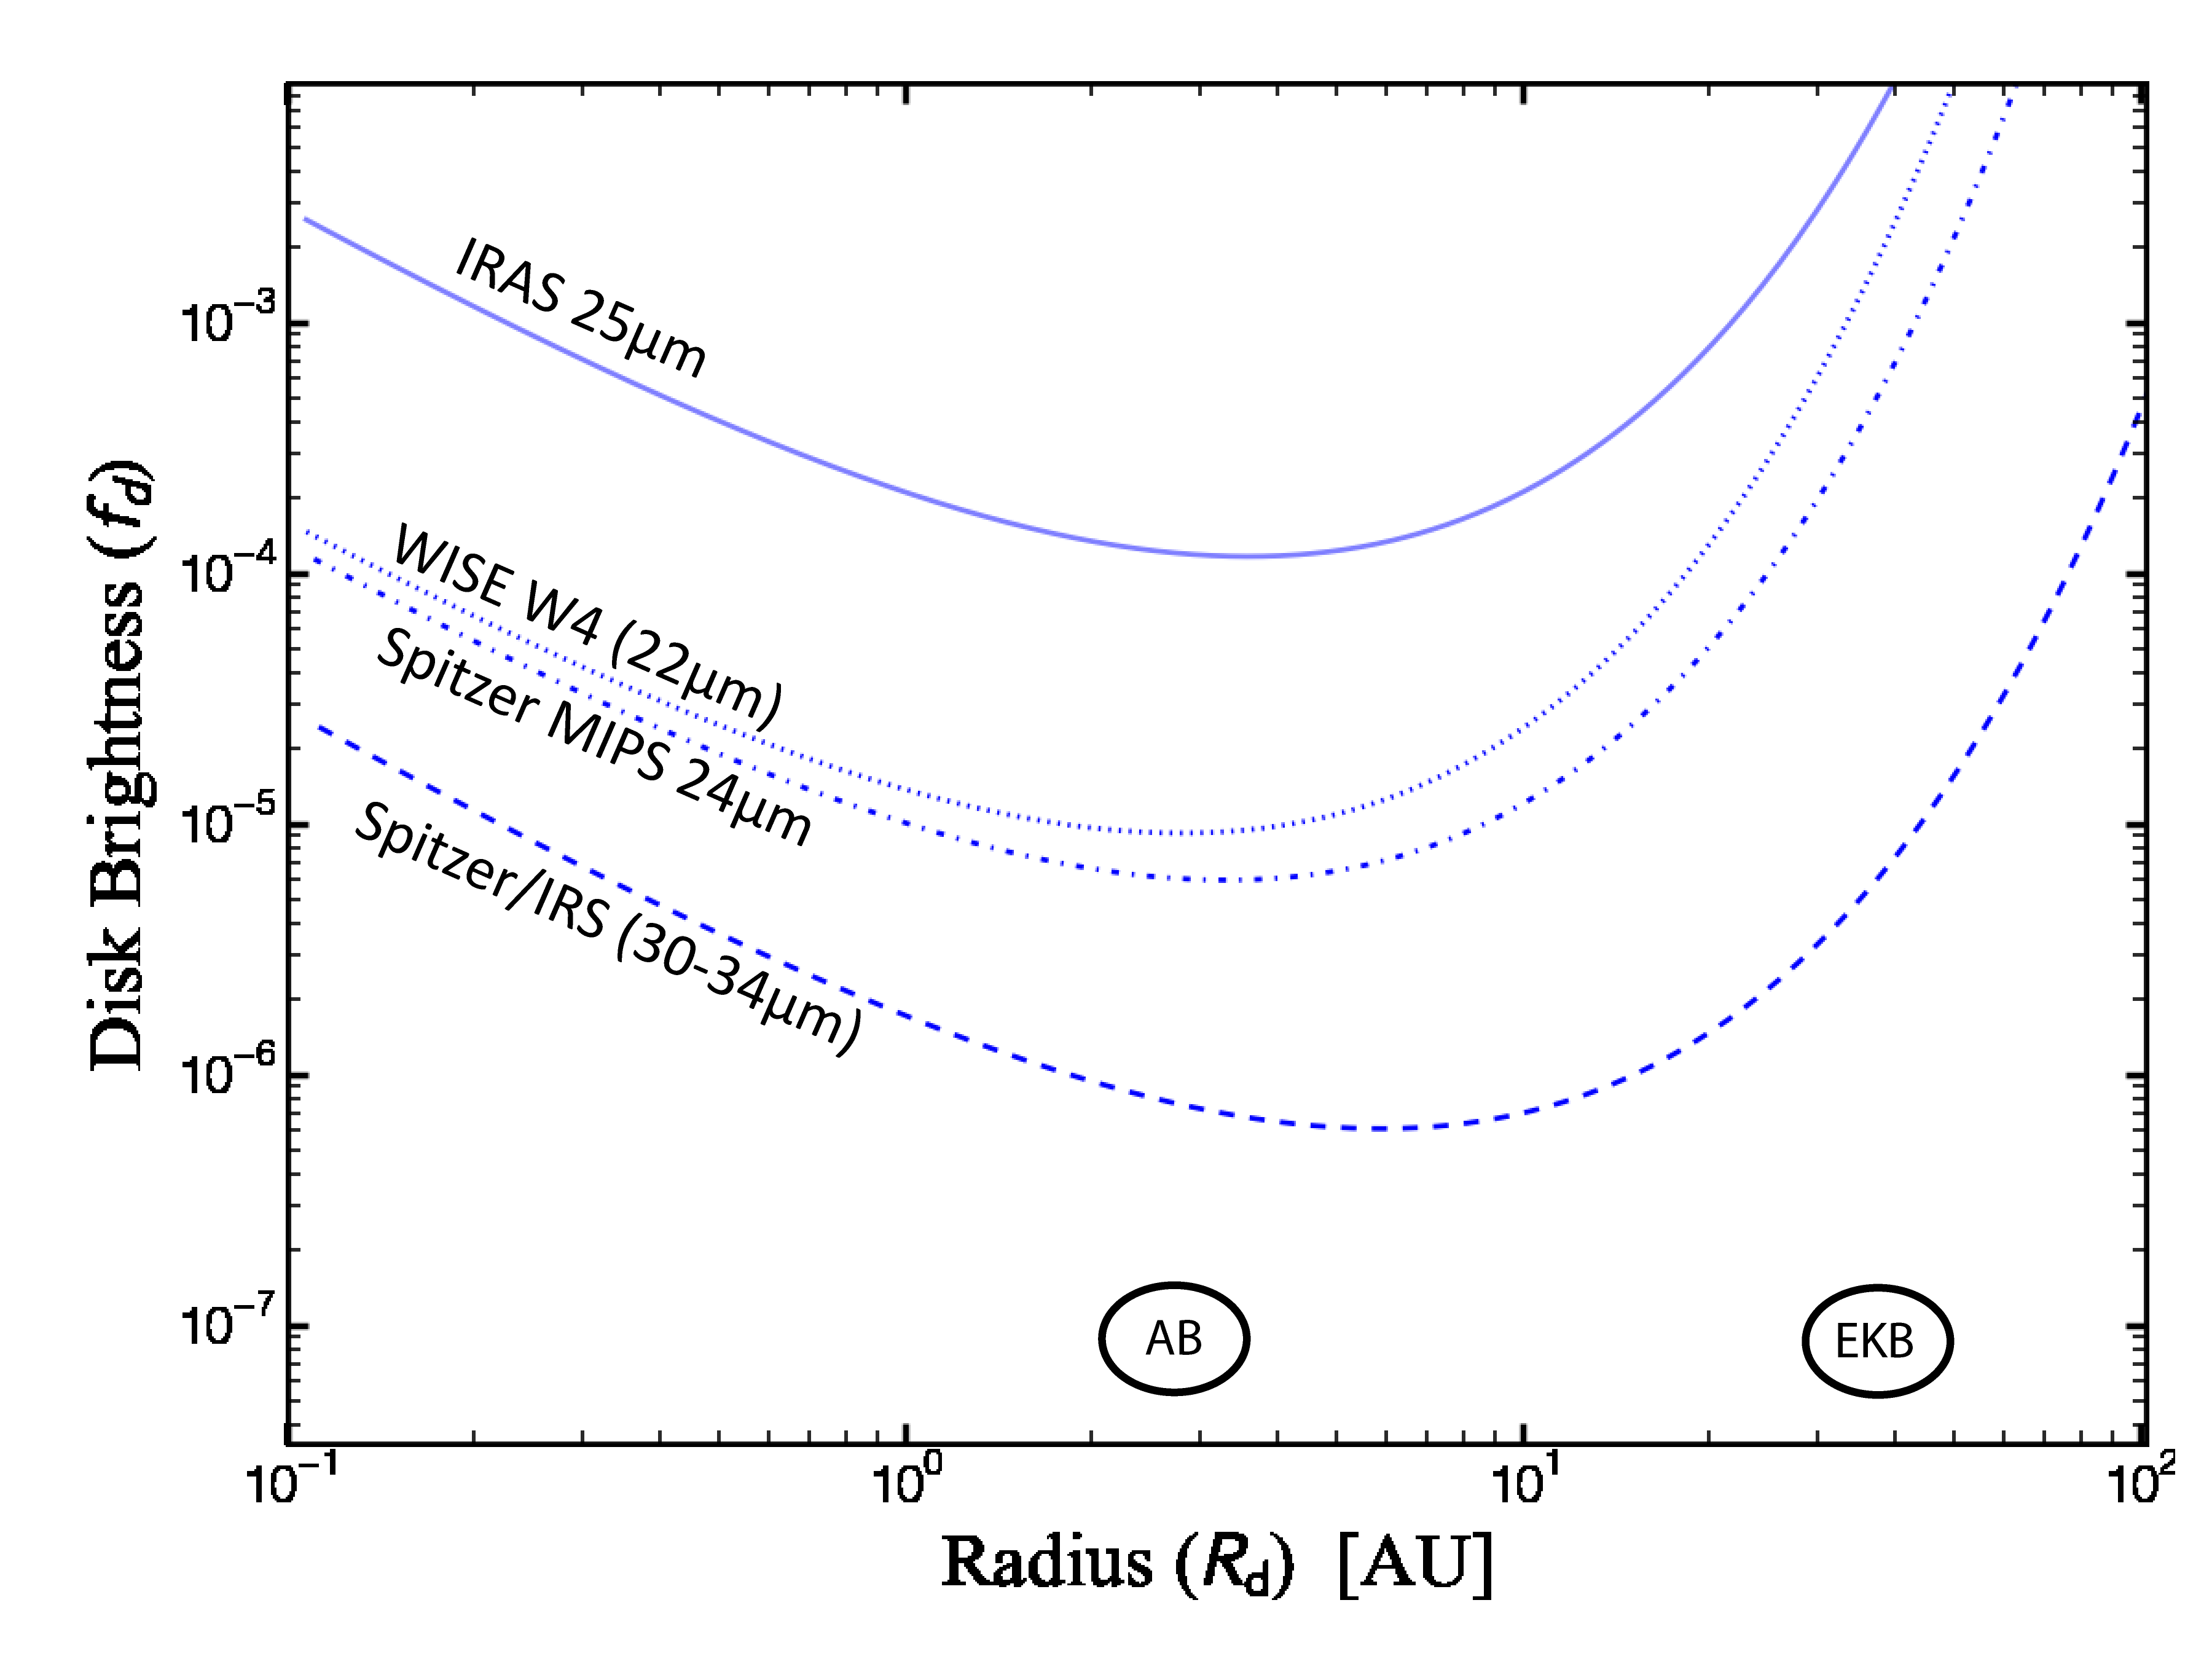
\includegraphics[scale=0.5]{Ch2/fdd_vs_tbb}
    \caption[]{}
    \label{fig:sensitivity_all}
    \end{figure}
    %===================================================================

    
    
    The size of the WISE All-Sky Database is also important because it provides an advantage over surveys that use Spitzer or Herschel to search for excesses. Figure~\ref{fig:sensitivity_all} compares the projected sensitivity of instruments on board WISE, Spitzer, and \iras\ in the mid-IR. While it is clear that WISE is able to detect fainter dust than \iras\ at similar wavelength bands, The Spitzer/MIPS and IRS instruments have been used to find even fainter dust populations. This is no surprise because Spitzer is a pointed survey, with higher angular resolution than WISE, and can hence increase its sensitivity to fainter dust through longer observing times. But, since pointed surveys can only observe a tiny fraction of the sky, the data products from an all-sky survey, like WISE, can search for excesses around stars which have never been observed. 
    
    
    
\section{Detecting Thermal Emission From Debris Disks with WISE}

    \subsection{Advantages of WISE Color Excess}\label{sec:advantage_wise}
    
    Most debris disks have been found from the subtraction of the measured IR flux from the modelled photospheric flux, as described in \S~\textbf{find appro. section}. An alternative to photospheric modelling of individual stars is to derive an estimate of the excess empirically by calculating star's ``color excess''. The astronomical magnitude system defines the color of a star by the logarithmic ratio of fluxes at two different wavelengths
    
    \begin{equation}\label{eq:color}
    m_{\lambda_1} - m_{\lambda_2} = -2.5\log{F_{\lambda_1}/F_{\lambda_2}},
    \end{equation}
    
    \noindent where $\lambda_1<\lambda_2$. For our purposes, we will assume that $\lambda_1$ is between $2-5$\micron\ and $\lambda_2>10$\micron. If we knew the ``photospheric color'', (i.e., color of the dust-free star) ${\left(m_{\lambda_1} - m_{\lambda_2}\right)}_\star$, then we can determine the color excess, by subtracting the photospheric color from the measured color ${\left(m_{\lambda_1} - m_{\lambda_2}\right)}_m$
    
    \begin{eqnarray}\label{eq:color_excess}
    E\left[m_{\lambda_1} - m_{\lambda_2}\right] &=& {\left(m_{\lambda_1} - m_{\lambda_2}\right)}_m - {\left(m_{\lambda_1} - m_{\lambda_2}\right)}_\star \\ 
    &=& {m_{\lambda_2}}_\star - {m_{\lambda_2}}_m,
    \end{eqnarray}
    
    \noindent where we assume that ${m_{\lambda_1}}_\star = {m_{\lambda_1}}_m$, and that the photospheric color is estimated empirically from the average or median value of a large set of measurements. For photospheric colors, consistent with a Rayleigh-Jeans slope, $E\left[m_{\lambda_1} - m_{\lambda_2}\right]=0$. Thus, stars with excesses can be identified by positive, non-zero color excesses such that $E\left[m_{\lambda_1} - m_{\lambda_2}\right]>0$. 
    
    
    Searching for excesses by using color excesses can be advantageous over searching for excesses from photospheric fitting. The latter technique can introduce inherent biases in measuring the ``hidden'' dust emission. The photospheric emission in the IR is estimated from fitting a set of grid models using photometric or spectroscopic data from observations at different epochs. Intrinsic stellar variability will offset any extrapolated flux in the IR, subsequently over or even underestimating the amount of IR excess flux. But more importantly, by using data from multiple epochs and different instruments, the relative systematic uncertainties between the flux measurements will reduce the signal of the dust emission one is trying to extract.
    
    However, if the photospheric extrapolation is done by fitting contemporaneously obtained data from the same instrument, the relative systematic uncertainties disappear. For example, \citet{Lawler2009} conducted a study that used contemporaneous Spitzer/IRS spectra. By using the shorter wavelength end of the spectra as an anchor for the photospheric emission, they were then able to extrapolate it to the relevant excess wavelengths. Most surveys are not afforded this luxury of simultaneous data in short and long wavelength observations, and hence SED fitting is the primary method. The difference in the flux of the detected excess between ``color excesses'' and ``photospheric fitting'' is small and only becomes relevant when searching for faint excesses ($f_d < 10^{-5}$--$10^{-7}$). Though when the goal is to attain greater sensitivity to solar system like dust ($f_d\sim10^{-7}$), the added sensitivity can go a long way.
    
    It is in this regime that WISE has the largest advantage. For the first time, WISE has afforded astronomers the ability to conduct an IR excess search of debris disks through photometric data obtained contemporaneously at photospheric and excess relevant wavelengths \textit{of the entire sky}. Thus, it only makes sense to take advantage of the properties of this data and search for IR excesses using the more sensitive color excess search technique. In this case, equation~\ref{eq:color_excess} will look like
    
    \begin{equation}\label{eq:wise_color_excess}
    E\left[Wi - Wj\right] = {\left(Wi - Wj \right)}_m - {\left(Wi- Wj \right)}_\star , 
    \end{equation}
    
    
 \noindent where $Wi$ and $Wj$ are the WISE bands described in \S~\ref{sec:wise_bands}, such that $Wi$ = $W1$, $W2$, or $W3$ and $Wj$ = $W3$ or $W4$ with the constraint that $Wi<Wj$. The work that I will present in the rest of this thesis is based on the measurements defined in equation~\ref{eq:wise_color_excess}. By using the color excess technique in conjunction with the all-sky coverage data from WISE, I will not only be able to identify a large number of excesses but also gain sensitivity to fainter warm disks  around stars that were previously missed due to either lack of resolution or coverage. 
    


    
\section{Previous \WS\ Debris Disk Studies}

    The series of studies I will be presenting in the subsequent chapters are by no means the first or only studies that have searched for debris disks using data from \WS. Here, I will summarize the current literature of \WS\ studies to detect debris disks.
    
    Studies have used data from different data releases on a variety of different data sets to search for debris disks. In particular, a number of studies have searched for excesses around different sets of exoplanet populations to study the relationship between the two. \citet{Krivov2011} and \citet{Morales2012} determined that $\sim$2\% of known exoplanet transiting hosts possess warm dust based on the \WS\ $W3$ or $W4$ excesses. \citet{Kennedy2012}, \citet{Ribas2012}, and \citet{Lawler2012} searched for excesses around stars in the \textit{Kepler} field. Altogether, roughly two dozen stars with $W3$ or $W4$ excesses were identified. 
    
    Other studies aimed to study the evolution of disks around a younger set of stars. The Scorpius-Centaurus OB association was heavily scrutinized by \citet{Rizzuto2012}, \citet{Luhman2012}, and \citet{Riaz2012}. About 150 stars with excesses were identified from these studies. Other studies focused on \WS\ debris disk searches for sets of spectral types around stars in the solar neighborhood. \citet{Avenhaus2012} found no significant \WS\ excess flux around 103 M-dwarfs, while \citet{Vican2014} identified 98 excesses from a sample of $\sim$8800 solar type stars. 
    
    \citet{Wu2013} and \citet{Kennedy2013} searched for excesses around a larger, unbiased sample of stars. The latter study searched for $W3$ excesses, around main-sequence \hip\ stars, while the former study searched for $W4$ excesses around the same set of stars. \citet{Kennedy2013} found 7 new $W3$ excesses with an incidence rate of $<1$\% for warm dust in the habitable zone of main sequence stars. \citet{Wu2013} identified roughly 70 new bright $W4$ excesses for stars out to 200~pc. In total, roughly 250 new excesses were identified by all these studies using data from \WS. These studies have increased our understanding of warm dust, and how it relates to systems of different ages, as well as systems with known planets. 
    
    However, there are inherent biases and limitations in the aforementioned studies, such that the true potential of searching for excesses with the \WS\ database is not realized \textbf{reword}. One drawback is in the sample sizes used in some of these studies. However, the size of the sample is often time unavoidable (e.g., due to $\sim$ only 1500 known exoplanets, or dearth of nearby young stellar associations). A greater concern is in the methods used to identify excesses. For instance, the majority of these surveys identified excesses by using SED fitting. This technique is prone to identifying a large number of bright excesses, based on the discussion in \S~\ref{sec:advantage_wise}. The rest of the studies identified excesses based on the \WS\ colors alone, without having subtracted off the photospheric \WS\ color. This also leads to identifying inherently bright excesses, but can also introduce large false-positve detections without proper subtraction of the photospheric color. One other bias, as discussed in \S~\ref{sec:bad_wise}, the \WS\ bands saturate at relatively faint magnitudes. And since all of these surveys did not include these saturated stars in their search, they are incomplete for relatively nearby stars. 
    
    In the following chapters, I will address these biases and present a set of studies that complements, as well as improves upon the search for warm dust with \WS. I utilize the \WS\ data to accurately understand the systematic behavior of the \WS\ data and identify warm dust around nearby main-sequence stars through the use of empirically identified \WS\ colors in addition to incorporating bright, saturated \WS\ photometry. Thus, not only are we able to find faint warm dust in some of these systems, relative to published studies, it will search for undetected excesses around nearby bright stars. 
    
    
    